% main.tex -- ClosetTwin business plan (assignment 02). Build from the root:
%   lualatex --disable-installer main ; biber main ; lualatex --disable-installer main (twice)
% Assembled by fix-se under the exception recorded in PLAN.md (owner: master-se).
\documentclass{closettwin}

\ctbrand{ClosetTwin}
\ctbibresource{references.bib}

\cttitle{ClosetTwin}
\ctsubtitle{An AI virtual fitting room for fashion e-commerce}
\ctdoctype{Business plan · 2026}
\ctauthors{Hila Abay, Shirel Giladi}
\ctgroup{sg00ha11}
\ctcourse{Generative AI for Management}
\ctlecturer{Dr. Yoram Segal}
\ctdate{November 2026}

\begin{document}

\frontmatter
\ctmakecover
\begin{hebrewpage}[תקציר מנהלים]
\hebtitle{תקציר מנהלים}

\hebsubtitle{ClosetTwin: חדר הלבשה וירטואלי מבוסס AI}

ClosetTwin היא חברת B2B שמציעה לאתרי אופנה חדר הלבשה וירטואלי מבוסס AI: סריקת גוף מהטלפון, מידות הבגד ונטיית ההתאמה של הקונה מתחברות להמלצה על מידה. החזרות עולות לקמעונאים בארצות הברית בין 685 ל-890 מיליארד דולר ב-\range{2024}{2024}, לפי שתי הערכות שונות (Appriss ו-NRF). בסקר של Coresight הוחזרו \pct{24.4} מההזמנות המקוונות של ביגוד, ו-\pct{53} מהמשיבים ציינו מידה והתאמה כסיבה המרכזית. מחיר החזרה הוא כ-\pct{17} מעלות הייצור (במקרה של נעליים).

שוק חדרי ההלבשה הווירטואליים מוערך ב-8.5 מיליארד דולר ב-2025 (IMARC), אך זו הערכה של מו״ל ללא שיטה פומבית. המסחר המקוון בישראל מוערך ב-6.9 מיליארד דולר ב-2024, ואופנה היא הקטגוריה הגדולה בו. השוק הישראלי קטן: סך דמי השימוש האפשריים אצל קמעונאים מקומיים הוא כ-0.2 מיליון דולר בשנה, ולכן ישראל היא שוק הוכחה ואירופה, מהשנה הרביעית, נושאת את ההכנסות.

המחיר המוערך הוא 0.036 דולר להזמנה (כ-\ils{0.13}). הטענה המרכזית היא השערה, ולא עובדה: פיילוט אקראי של 4 שבועות יכול לגלות ירידה של כ-\pct{7.8} בהחזרות אצל קמעונאי ישראלי גדול. כלל הפרטיות העיקרי הוא תיקון 13 לחוק הגנת הפרטיות (בתוקף מאז 14 באוגוסט 2025): מזהה ביומטרי הוא מידע רגיש רק כשהוא משמש לזיהוי אדם, ו-ClosetTwin סורקת להתאמת מידה ולא לזיהוי. תקנות GDPR משניות ורלוונטיות בשלב אירופה.

אין רווח תפעולי בחמש השנים הראשונות. מסמך זה מתוארך ל-2026, והגיוס המבוקש הוא כ-2.8 מיליון דולר (ערך נגזר והנחה, שיתעדכן מהמודל). ערוץ המכירה הראשון הוא מכירה ישירה לקמעונאי אופנה מקומיים, ומשנה רביעית באירופה, גם דרך Shopify.
\end{hebrewpage}

\tableofcontents
\listoffigures
\listoftables

\mainmatter
\chapter{Introduction and Problem}\label{ch:intro}

\statcard{\$685\,B--\$890\,B}{Returns of the US retail industry in 2024, by two different methods}{Sources: Appriss Retail \cite{appriss2024}; NRF \cite{nrf2024}}
\statcard{24.4\%}{Online apparel orders returned in the 12 months to March 2023 (US survey of 100 decision-makers)}{Source: Coresight Research \cite{coresight2023}}
\statcard{53\%}{Surveyed decision-makers who name size or fit the top reason for apparel returns}{Source: Coresight Research \cite{coresight2023}; share of respondents, not of returns}
\statcard{17\%}{Cost of one return as a share of the prime cost (one Scandinavian footwear retailer)}{Source: Gustafsson et al. \cite{gustafsson2021}}

\section{The returns bill}\label{sec:returns-bill}

Every order that comes back is a sale that did not finish and a cost that did. The two best estimates of what this costs retailers in the United States are large and differ from each other. Appriss Retail reports that total returns of the retail industry amounted to \$685 billion in merchandise in 2024, and the National Retail Federation projects \$890 billion for the same year \cite{appriss2024,nrf2024}. The gap of \$205 billion is a difference of method and not a contradiction. The Appriss figure is built from surveys of 150 North American retail executives and 1,000 consumers together with data of the US Census Bureau, while the NRF figure is a projection published on the federation's report page \cite{appriss2024,nrf2024}. We therefore quote the range and not a single number, and we do not add the two. Appriss also reports that online sales account for \$362 billion of the returned value and that fraud and abuse account for 15.14\% of all returns \cite{appriss2024}. The second figure matters for honesty: not every return is a fit problem, and a fitting tool cannot reduce fraud.

Two different return rates circulate in the trade press, and they must not be merged. Appriss reports that online returns reached 24.52\% of all online sales, which covers every product category \cite{appriss2024}. Coresight Research estimates that the average return rate of online apparel orders was 24.4\% for the twelve months ended March 2023, from a survey of 100 decision-makers at US apparel brands and retailers \cite{coresight2023}. The similarity of the two numbers is a coincidence of two scopes. This plan uses the Coresight figure, because it is the one that is specific to apparel, and it states each time that the base is a small US survey.

\section{Why fit is the core cause}\label{sec:fit-cause}

Among the reasons for apparel returns, size and fit come first. In the Coresight survey, 53\% of respondents name size or fit as the top reason for online apparel returns, followed by color (16\%) and damage (10\%) \cite{coresight2023}. This is a share of respondents and not a share of returns, and the plan treats it that way: our own model assumes that 40\% of returns are fit-related, which is a deliberate step below the survey figure (Chapter~\ref{ch:finance}). The same picture appears in the research literature. Abdulla et al. state that online shopping yields a large percentage of returns due to size and fit \cite{abdulla2019}, and Alemany et al. describe the high number of returns and their management, logistics and operating costs as an important economic burden for fashion companies \cite{alemany2013}. Peng and Duraffourg report that the return rate in the textile industry is in general between 20\% and 40\%, a secondary claim that they make without a citation in their abstract \cite{peng2023}.

The literature also tells us what kind of problem this is. A shopper who orders online cannot try the garment on, so the decision is made on incomplete information: the shopper knows his or her body only roughly, and the garment is described by a size label that means different things at different brands. Alemany et al. note that earlier fitting technologies did not reach a compromise between cost, efficacy and accuracy that would allow wide market penetration \cite{alemany2013}, and we treat this as the historical gap that a lower-cost scan and a data-driven model can address. In a different field, Pfaff and Spann report that augmented reality is particularly effective for larger products with higher spatial fit uncertainty \cite{pfaff2025}. We cite it only as an analogy: the study is about home interiors and not about apparel.

\section{What one return costs}\label{sec:return-cost}

A return is expensive because it is handled twice. In the one study that built the cost of a return from transaction data, 2,229 return transactions of a Scandinavian fashion footwear retailer, the cost of a return is approximately 17\% of the prime cost, and product handling and transportation together make up 72\% of that cost \cite{gustafsson2021}. This is a single retailer and a single product category, so it is an anchor for the model and not a market constant. Coresight estimates, for the United States, that a 24.4\% return rate on a \$155.8 billion online apparel and footwear market translates to \$38 billion in returns and \$25.1 billion in processing costs in 2023 \cite{coresight2023}. We use the Gustafsson ratio in our model and show the Coresight figures only as a statement of scale.

For Israel, which is the first market of this plan, the legal setting makes returns structurally material. According to the official guide of the Israeli Consumer Protection and Fair Trade Authority, a consumer may cancel a distance-selling transaction within fourteen days of closing the transaction or of receiving the document with its details, whichever is later; use of the product does not remove the right, and the business must refund the consumer within fourteen days of receiving the cancellation notice \cite{il_cpfta_guide}. The business may charge a cancellation fee of 5\% of the transaction or NIS~100, whichever is lower, and may not charge it when the product is defective or differs from the details provided \cite{il_cpfta_guide}. We found no verified Israeli return rate. The plan's return rate therefore stays at the US figure of \assumed{24.4\%}, and it is an assumption anchored on a US survey and not Israeli data.

\section{The thesis and how this plan tests it}\label{sec:thesis}

ClosetTwin is a business-to-business virtual fitting room for fashion e-commerce. The shopper gives a body scan from a phone, the retailer supplies the garment's measurements, and the service combines both with the shopper's stated fit preference to recommend a size. The claim at the center of the plan is a hypothesis and not a fact: \emph{a fit tool built on scan, garment data and preference lowers fit-related returns enough to pay for itself}. The evidence is mixed. Gustafsson et al. model reductions of fit-related return costs of up to 80\% under assumed verification rates, but this is a scenario \cite{gustafsson2021}. The largest field study in our sources, covering 496,365 items ordered by 75,707 customers, found that customers who used a size finder were 0.65\% more likely to return an item, although their customer lifetime value was higher \cite{patel2025}. A plan that ignored the second result would be dishonest.

The plan therefore treats the effect as the quantity to be measured. Chapter~\ref{ch:market} sizes the market and finds that Israel alone is too small to carry the company. Chapter~\ref{ch:competition} places ClosetTwin among the existing vendors. Chapters~\ref{ch:product} and~\ref{ch:business} describe the product and its pricing, which is set at a fraction of the value a retailer saves if the hypothesis holds. Chapter~\ref{ch:gtm} designs a randomized pilot that can accept or reject the hypothesis, and Chapters~\ref{ch:finance} to~\ref{ch:conclusion} show what the company costs, what it earns and what it asks for if the pilot passes. Where a number is our own, it is marked as derived or assumed, and the legend is \ctlegend{}.

\ctchapterend

\chapter{Market: TAM, SAM and SOM}\label{ch:market}

\section{Method and its limits}\label{sec:market-method}

We size the market bottom-up, in orders and in the fee that ClosetTwin would earn on them, and we call the result a \emph{fee pool} and not a market size. A fee pool is the number of orders a segment could send through the service multiplied by our blended price, so it measures what we could earn and not what retailers or shoppers spend. Each input carries one of three marks: sourced, derived by us from other inputs, or assumed by us with a stated basis (\ctlegend{}). Table~\ref{tab:sam-inputs} lists them all.

The Israeli figures need a warning. The market numbers come from Statista estimates that a research report of the Knesset Research and Information Center relays \cite{knesset_ric2025}. They are not a release of the Central Bureau of Statistics, the 2024 value is an estimate, and the fashion share is the 2022 value. Publisher estimates of the virtual-fitting-room market are context only and enter no calculation: IMARC Group reports that this global market reached \$8.5 billion in 2025 and will reach \$52.6 billion by 2034, a compound annual growth rate of 21.80\% \cite{imarc2026}, but the definition and method sit in a paid report that we could not read, and we found no second publisher that we could verify.

\section{Israeli online commerce in context}\label{sec:market-context}

Israeli online commerce is small next to the markets in which fitting vendors usually operate, but it is growing. The Knesset report, citing Statista, puts total online trade at about \$6.1 billion in 2023, or about NIS~22.6 billion, which is about 2.6\% of household private consumption; the estimate for 2024 is \$6.9 billion and the forecast for 2029 is \$11.3 billion \cite{knesset_ric2025}. The ratio of the two 2023 figures gives a rate of 3.70 shekels to the dollar, and we use this derived rate whenever a shekel equivalent is shown, for example \$0.036 per order, which is about \ils{0.13}. Fashion is the largest online category: in 2022 it was about 21.6\% of Israeli online commerce, ahead of electronics at about 20\% \cite{knesset_ric2025}.

\section{TAM: Israeli online fashion}\label{sec:tam}

For the total addressable market we take the 2022 fashion share of 21.6\% and hold it at its 2022 value for 2024, which gives \derived{\$1.49 billion} of online fashion sales in Israel, about NIS~5.5 billion. We multiply the share and not the shekel figure for 2022 because the report's own 2022 figures imply a rate of 3.37 shekels to the dollar, and a 2022 shekel value converted at the 2023 rate would mix two years. At an assumed average order value of \assumed{\$80} this is \derived{18.6 million} online fashion orders a year. At the blended price of \$0.036 per order, the fee pool of the whole Israeli online fashion market is only \derived{\$0.67 million} a year.

\section{SAM: local Israeli e-tailers only}\label{sec:sam}

The serviceable market is smaller still. Foreign sites are prominent among the sellers that Israeli shoppers use. The 2020 sales ranking in the Knesset report is led by Amazon with \$195 million, followed by Shein (\$151 million), and it also lists Next (\$96 million), ASOS (\$57 million) and Zara (\$51 million) \cite{knesset_ric2025}. The same report adds two charts by share of orders from November 2024, which it takes from Statista. Among global sites, AliExpress leads with 57\%, followed by Shein (12\%), Amazon and Temu (7\% each) and Next (5\%); among local sites, Super-Pharm leads with 22\%, followed by Shufersal (20\%), KSP (15\%) and Terminal X (12\%) \cite{knesset_ric2025}. The charts are two separate rankings and the report does not classify the sites by category, so they do not give a split of fashion orders between local and foreign sites. A foreign site that serves Israeli shoppers will not buy a plug-in from an Israeli start-up for that market. We therefore assume that \assumed{45\%} of Israeli online fashion orders go to local e-tailers, which is \derived{8.4 million} orders. The order shares above name individual local sites but give no number of orders for any Israeli fashion e-tailer, so we assume three size bands: 5 large retailers with 600,000 orders a year each, 25 mid-size retailers with 100,000 each and 250 small shops with 12,000 each. The bands add up to 8.5 million orders, within 2\% of the 8.4 million above. We address the large and mid-size retailers only, since a shop with 12,000 orders pays about \$430 a year and cannot justify an integration. That leaves 30 candidate retailers and \derived{5.5 million} orders, a fee pool of \derived{\$198,000} a year.

\begin{insightbox}[Israel is a reference market, not a revenue market]
The Israeli SAM fee pool is about \$0.2 million a year. No team can live on that. The Israeli plan is therefore a strategy for reference customers, for pilots that can prove the effect, and for early learning. Revenue must come from Europe.
\end{insightbox}

Why start in a market this small? There are three reasons, and none of them is revenue. First, the plan's central hypothesis can be tested only with a real retailer, and the five large Israeli retailers of our bands have enough orders for an individual test (Chapter~\ref{ch:gtm}). Second, a pilot is cheap: we assume a cash cost of \assumed{\$3,000} for a direct pilot (Chapter~\ref{ch:finance}). Third, Israeli retailers work under a statutory 14-day cancellation right (Chapter~\ref{ch:intro}), so returns are a real cost to them. The price of this choice is stated openly: by the model, the cumulative operating result at the end of year~3, before Europe opens, is a deficit of \derived{\$1.04 million}, spent in a market whose whole SAM is about \$0.2 million a year. A reference customer in Israel is useful in Europe only if European retailers accept it, and we have no evidence of that. The model does not include a route to Europe through Israeli retailers that sell to EU customers; its European clients are European retailers that the sales team reaches directly.

\begin{table}
\caption{Inputs of the market sizing, with the class of each}\label{tab:sam-inputs}
\begin{tabularx}{\textwidth}{lrlX}
\toprule
\ctheaderrow\cthead{Input} & \cthead{Value} & \cthead{Class} & \cthead{Source or basis}\\
\midrule
Online commerce 2024 & \$6.9\,B & sourced & Knesset report \cite{knesset_ric2025}\\
Fashion share, 2022 & 21.6\% & sourced & same report\\
Online fashion sales 2024 & \$1.49\,B & derived & share $\times$ \$6.9\,B\\
Average order value & \$80 & assumed & mid-market basket\\
Online fashion orders & 18.6\,M & derived & sales $\div$ order value\\
Share going to local e-tailers & 45\% & assumed & largest sites are foreign\\
Retailers (large / mid / small) & 5 / 25 / 250 & assumed & bands; order shares only in the report\\
SAM orders (large and mid) & 5.5\,M & derived & 5 $\times$ 600,000 + 25 $\times$ 100,000\\
Blended price per order & \$0.036 & derived & 60\% at \$0.04, 40\% at \$0.03\\
Israeli SAM fee pool & \$198,000 & derived & SAM orders $\times$ price\\
Europe share of global apparel & 25\% & assumed & non-APAC is 57.3\%\\
Global e-commerce apparel 2024 & \$726\,B & sourced & Kings Research \cite{kings2026}\\
Europe fee pool (TAM / SAM) & \$81.7\,M / \$32.7\,M & derived & orders $\times$ price; SAM at 40\%\\
\bottomrule
\end{tabularx}
\end{table}

\begin{figure}
% F1: TAM / SAM / SOM, Israel (nested) and Europe layer (separate). Not to scale.
% No caption/label here: the chapter owns them (fig:f1).
% Numbers: python/model.py D30, D34b_tam, D33, D34, SUBI_5, D35, D36, D37, SUBE_5. D = derived.
\begin{tikzpicture}[x=0.37cm,y=0.4cm]
  \node[ct title,anchor=south west] at (0,16.1) {Israel (beachhead)};
  \draw[ct node ivory] (0,0) rectangle (17.5,16);
  \node[ct label,anchor=north west,align=left] at (0.4,15.7)
    {\textbf{TAM} online fashion: 18.6\,M orders,\\fee pool \$0.67\,M a year\textsuperscript{D}};
  \draw[ct node pink,minimum width=0pt] (1,1) rectangle (16.5,10.8);
  \node[ct label,anchor=north west,align=left] at (1.4,10.5)
    {\textbf{SAM} local e-tailers, large and mid:\\5.5\,M orders, fee pool \$0.20\,M a year\textsuperscript{D}};
  \draw[ct key,minimum width=0pt] (2.3,2) rectangle (15.2,5.8);
  \node[ct label,text=ivory,align=center] at (8.75,3.9)
    {\textbf{SOM}, year 5\\Israeli subscription \$54\,k\textsuperscript{D}};

  \node[ct title,anchor=south west] at (20,16.1) {Europe layer (from year 4)};
  \draw[ct node ivory,dashed] (20,5.5) rectangle (37.5,16);
  \node[ct label,anchor=north west,align=left] at (20.4,15.7)
    {\textbf{TAM} 2.27\,B orders,\\fee pool \$81.7\,M a year\textsuperscript{D}};
  \draw[ct node pink,dashed,minimum width=0pt] (21,6.5) rectangle (36.5,11.2);
  \node[ct label,anchor=north west,align=left] at (21.4,10.9)
    {\textbf{SAM} fee pool\\\$32.7\,M a year\textsuperscript{D}};
  \draw[ct key,minimum width=0pt] (21,0.5) rectangle (36.5,4.5);
  \node[ct label,text=ivory,align=center] at (28.75,2.5)
    {\textbf{SOM}, year 5: subscription \$0.32\,M\textsuperscript{D}\\(not in the Y1--Y3 base case)};
\end{tikzpicture}

\caption{Market layers, not to scale: Israel (nested TAM, SAM, SOM) and the Europe layer; fee pools per year}\label{fig:f1}
\end{figure}

\section{Europe layer and SOM}\label{sec:europe-som}

Because the Israeli SAM cannot fund a team, Israel is the proof market, and Europe, entered in year 4, carries the revenue (Figure~\ref{fig:f1}). Kings Research values the global e-commerce apparel market at \$726.05 billion in 2024, of which Asia-Pacific holds 42.70\% \cite{kings2026}. The remaining 57.3\% is divided between North America, Europe and the rest of the world in a way that no source we hold gives, so we assume that Europe holds \assumed{25\%} of the global total. Divided by the same \$80 order, this is \derived{2.27 billion} orders and, at the blended price, a Europe fee pool of \derived{\$81.7 million} a year. Applying the same 40\% size filter that excludes marketplaces and small shops, which we assume for Europe only, leaves a Europe SAM of \derived{\$32.7 million}. Together with the Israeli SAM, the combined serviceable pool is \$32.9 million a year. Europe is not part of the base case of the first three years, and the plan does not claim revenue there before year~5.

The serviceable obtainable market (SOM) is the part of that pool the plan expects to win by year~5. Total revenue in year~5 is \derived{\$782,000}. Of this, Israeli subscription revenue is only \$54,000, European subscription revenue is \$648,000 and pilot fees make up the rest (Chapter~\ref{ch:finance}). Subscription revenue alone is 2.1\% of the combined SAM. This is a modest share, and the plan deliberately asks for a small slice of a pool that is still large enough to support a company. The weak link is not the size of the share but the assumption behind it, that half of the pilots become paying clients; Chapter~\ref{ch:gtm} says how the pilots test it.

\ctchapterend

\chapter{Competition}\label{ch:competition}

\section{How to read the table}\label{sec:comp-read}

Table~\ref{tab:vendors} lists what each vendor says about itself on its own public pages, which we read on 18 November 2026. Everything in it is a vendor claim, and none of it is independent evidence. A cell that reads ``not stated'' means that the page we could read does not say; it does not mean that the vendor lacks the feature. Prices are left out of the table because none of these vendors publishes one for its retail product; Chapter~\ref{ch:business} discusses the one public price list. Pages change, so the table is a snapshot.

\begin{table}
\caption{Vendor claims, as stated by the vendors (a snapshot)}\label{tab:vendors}
\begin{tabularx}{\textwidth}{lXX}
\toprule
\ctheaderrow\cthead{Vendor} & \cthead{What the vendor states} & \cthead{Shopper input}\\
\midrule
True Fit \cite{truefit_web} & fit and sizing intelligence, built on 20 years of purchase and return outcomes & purchase and return history; scanning not mentioned\\
Fit Analytics \cite{fitanalytics_web} & machine-learning size and fit recommendations & preferences, sales and returns records, a database of body scans\\
3DLOOK \cite{threedlook_web} & body scanning embedded by API or SDK; over 80 measurements in under 45 seconds & two guided smartphone photos \cite{threedlook_pricing}\\
Bold Metrics \cite{boldmetrics_web} & over 50 points of measure matched to the retailer's garment data & 4 to 6 simple inputs; no scanning, photos or tape\\
MySize \cite{mysize_web} & omnichannel platform with AI-driven apparel sizing & not stated\\
\midrule
Google \cite{google2023tryon} & generative-AI try-on on real models, sizes XXS to 4XL & a clothing image\\
Walmart and Zeekit \cite{walmart2021zeekit} & shoppers see themselves in a garment & uploaded photo or chosen model\\
\bottomrule
\end{tabularx}
\end{table}

\section{Direct vendors}\label{sec:comp-direct}

The direct field splits on one question: does the shopper scan, give a few inputs, or give nothing? True Fit sells to retailers and turns purchase-and-return outcomes into guidance, and its page does not mention body scanning \cite{truefit_web}. Fit Analytics states that it combines shopper preferences, sales and returns records with a database of body scans, so scans are reference data and not a shopper step \cite{fitanalytics_web}. 3DLOOK states that it embeds phone-based body scanning into a web page or app through an API, and its price list shows the cost of such scans \cite{threedlook_web,threedlook_pricing}. Bold Metrics takes the opposite position, stating that it needs no scanning, photos or measuring tape and works from four to six simple inputs \cite{boldmetrics_web}.

MySize is the one direct competitor at home. According to its annual report for 2022, the company is incorporated in Delaware, lists on the Nasdaq Capital Market and has its principal executive offices in Airport City, Israel \cite{mysize10k2022}. Its public page describes an omnichannel platform with AI-driven apparel sizing and says nothing we could check about scanning or price \cite{mysize_web}. We did not check whether the address has changed since 2022.

\section{Platform and in-house threats}\label{sec:comp-platform}

Large platforms are a different kind of threat. Google announced in 2023 a generative model that takes one clothing image and shows how it would drape on real models in sizes from XXS to 4XL \cite{google2023tryon}, and Walmart announced in 2021 a plan to acquire Zeekit, which lets customers see themselves in a garment from an uploaded picture or a chosen model \cite{walmart2021zeekit}. These tools visualize a garment, which is different from recommending a size, but a retailer that already has free visualization may feel that it does not need a vendor. We have not verified the later status of the Walmart plan.

\section{Positioning}\label{sec:comp-position}

Figure~\ref{fig:f2} places the vendors on two axes: whether the size comes from a questionnaire or size chart or from a body scan, and whether the product is a consumer app or a plug-in sold to retailers. ClosetTwin's chosen corner, a scan combined with garment specifications and fit preference, delivered as a plug-in to retailers, is not occupied by any vendor in the table. This proves only that the vendors do not say they occupy it; 3DLOOK, for one, could add the other inputs.

\begin{figure}
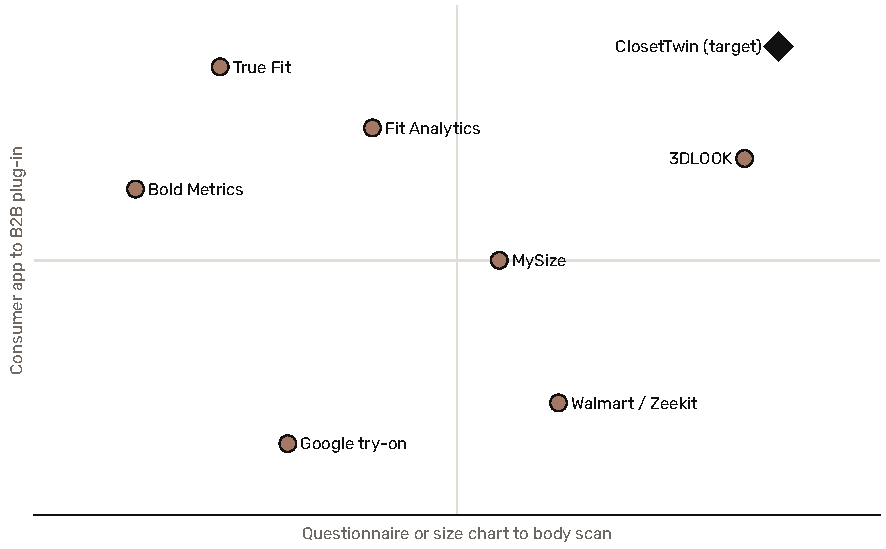
\includegraphics[width=\textwidth]{figures/f2-positioning.pdf}
\caption{Positioning of the vendors, our reading of vendor pages: source of the size input and type of product}\label{fig:f2}
\end{figure}

\section{The moat: proven, plausible or hypothesis}\label{sec:comp-moat}

We tag each claimed advantage honestly. That the combined input of scan, garment data and preference is better than any one of them is a \emph{hypothesis}: Peng and Duraffourg found that fit preference significantly affects the size people choose and that knowing the 3D shape alone is not enough for an efficient size recommendation \cite{peng2023}, which supports the combination but does not show that our implementation is better. That ClosetTwin lowers returns is a \emph{hypothesis until the pilot}. The counter-argument is real and we state it: Bold Metrics claims to match a shopper to garment data without a scan \cite{boldmetrics_web}, so a scan is an advantage only if it measurably improves the recommendation. Our edge in the early years is therefore a position and a test, not a moat.

\ctchapterend

\chapter{Product and Technology}\label{ch:product}

\section{What the shopper and the retailer see}\label{sec:product-see}

ClosetTwin is a widget on the retailer's product page and a data feed back to the retailer. The shopper opens the widget, takes two guided photographs with a phone, states how loose or fitted he or she likes the garment to be, and receives a recommended size for the garment on the page. The retailer sees the same process from the other side: it supplies the measurements of each garment, and in return it receives a stream of anonymous fit data, such as which sizes are recommended, which are bought and which come back. Figure~\ref{fig:f3} shows the flow from the scan to the retailer's data. The shopper never sees a three-dimensional avatar, because the first release is about choosing a size and not about visualization (Section~\ref{sec:product-viz}).

\begin{figure}
% F3: scan -> body model + garment specs + fit preference -> size -> retailer data flow.
% No caption/label here: the chapter owns them (fig:f3).
\begin{tikzpicture}[node distance=6mm and 9mm]
  \node[ct node ivory,minimum width=30mm] (scan) {Shopper scan\\(phone photos)};
  \node[ct node ivory,minimum width=30mm,below=of scan] (pref) {Fit preference\\(snug / loose)};
  \node[ct node ivory,minimum width=30mm,below=of pref] (spec) {Garment specs\\(from retailer)};
  \node[ct key,minimum width=26mm,right=14mm of pref] (model) {Body model\\+ fit engine};
  \node[ct node pink,minimum width=22mm,right=10mm of model] (size) {Recommended\\size};
  \node[ct node,minimum width=22mm,right=10mm of size] (shop) {Product page\\widget};
  \node[ct node ivory,minimum width=30mm,below=12mm of size] (feed) {Retailer data feed\\(sizes, returns)};
  \draw[ct arrow] (scan.east) -- ++(5mm,0) |- ([yshift=3mm]model.west);
  \draw[ct arrow] (pref.east) -- (model.west);
  \draw[ct arrow] (spec.east) -- ++(5mm,0) |- ([yshift=-3mm]model.west);
  \draw[ct arrow] (model) -- (size);
  \draw[ct arrow] (size) -- (shop);
  \draw[ct arrow] (shop.south) |- (feed.east);
  \draw[ct arrow,dashed] (feed.west) -| (spec.south);
\end{tikzpicture}

\caption{Data flow: scan, garment specifications and fit preference give a size and a retailer data feed}\label{fig:f3}
\end{figure}

\section{From scan to body model}\label{sec:product-scan}

A body model built from scan data is feasible and well studied, and the studies explain why it is needed. Alhassawi et al. analyzed a dataset of 677 participants and found that only 63 of them (9.15\%) kept the same size across bust, waist and hip, that 614 (90.84\%) fell into different sizes on different measurements, and that 35.45\% were not adequately accommodated by the existing sizing scheme \cite{alhassawi2025}. In other words, a single size label fits a minority of bodies on all dimensions at once. Alemany et al. made the same point earlier, and noted that body-scanning technologies at that time had not achieved a compromise between cost, efficacy and accuracy that would allow wide market penetration \cite{alemany2013}. That study is from 2013 and we cite it as history. What has changed is that phone-based capture now exists: 3DLOOK states that a user can complete a scan independently with two guided smartphone photos and no dedicated hardware \cite{threedlook_pricing}. This is a vendor statement, and it does not tell us how accurate such a scan is for apparel. We found no independent source for the accuracy of phone scans in apparel sizing, so we state it as an engineering target that the pilot must measure and not as a result.

\section{Why scan alone is not enough}\label{sec:product-pref}

A body measurement does not choose a size, because the same body can want different sizes in different garments. Peng and Duraffourg ran an experiment with 175 female participants of shapes from XS to 4XL on six garment tops. They report that fit preference has a significant impact on the size choice, and that knowing the three-dimensional shape of customers alone is not enough for an efficient size recommendation tool \cite{peng2023}. Two further findings, which we know only from their abstracts, point the same way. Sembium et al. report that latent-factor models that use personas and return codes improve the area under the curve by 17 to 21\% against baselines, and that in an online A/B test they raised the percentage of ``fit'' transactions by 0.49\% over the control \cite{sembium2017}. Zhang et al. report that thin models dissuade consumers with larger clothing sizes from buying online because of perceived body-size dissimilarity and a heightened perception of fit risk \cite{zhang2024}. The product therefore takes three inputs and not one: the scan, the garment's measurements and the shopper's stated preference. That the combination beats any single input is a hypothesis of this plan, which the pilot tests (Chapter~\ref{ch:gtm}).

\section{The size model and its accuracy limits}\label{sec:product-model}

The best evidence we hold for the model comes from a study on scan data that used the same kind of measurements. Alhassawi et al. report that a support vector machine that works on the primary measurements reaches an accuracy of 89.66\%, outperforming a model that adds further dimensions through principal-component analysis, which reaches 68.97\% \cite{alhassawi2025}. They also report that sizes 32 and 34 received no correct predictions, which they attribute to overlapping features and too few training samples \cite{alhassawi2025}. We take two lessons from this. First, a simple model on a few good measurements can be accurate enough to be worth testing. Second, the accuracy of such a model is lowest at the edges of the size range, so rare sizes need a fallback, for example a prompt to measure again or a note to the shopper that the recommendation is uncertain. We state the 89.66\% as the best evidence in hand and not as ClosetTwin's measured performance, because the study did not use our scans, our garments or our shoppers, and we have no measurement of our own yet.

\section{Integration with retailer platforms}\label{sec:product-integration}

Integration follows a standard pattern. On Shopify, an app is a set of components that the developer declares in the app configuration, and Shopify runs most of them, so that only the backend is the developer's to host \cite{shopify_dev_build}. A ClosetTwin app on that model needs a widget extension for the product page, a backend for the size model and a feed of the retailer's garment data. We have checked this pattern only for Shopify, which is a minor channel in Israel (Chapter~\ref{ch:gtm}); other platforms are not yet checked, and the plan does not assume that integration there is equally cheap. We assume \assumed{\$0.03} as the cost of one scan in our own infrastructure and \assumed{25\%} of orders that include a scan, which together give a cost to serve of \$0.0075 per order (Chapter~\ref{ch:business}).

\section{Privacy by design: scan for fit, not identification}\label{sec:privacy-design}

A body scan is personal data, and the product is designed so that it is not used for identification. Israel's Privacy Protection Law was amended by Amendment~13, published on 14 August 2024, and the amendment takes effect one year after publication, that is, on 14 August 2025 \cite{il_amend13_2024}. Under the law's definitions, a biometric identifier is data of special sensitivity when it is used, or intended to be used, to identify a person or to verify his or her identity in a digital manner \cite{il_amend13_2024,il_ppl_en}. ClosetTwin scans for fit only. The design therefore never uses body data to identify anyone, collects the minimum that the size model needs, keeps the scan separate from any account identity and, as a design rule, discards the images once the measurements are extracted. We offer explicit consent as \emph{our own design choice}: the law defines consent as informed consent, explicit or implied \cite{il_ppl_en}, so we do not claim that the law requires it. Whether body measurements for sizing could count as health data, which is a separate category of special sensitivity \cite{il_ppl_en}, is an open legal question. We treat it as a design risk that the compliance review must answer, not as a conclusion (Chapter~\ref{ch:risks}).

The regulator's own documents point the same way. The Privacy Protection Authority's 2021 draft opinion, published for public hearing, states that collecting excess data beyond what is necessary is in itself an infringement of privacy \cite{ppa_data_minimization2021}, and its 2025 guide to privacy-enhancing technologies says that building them into the design of systems supports compliance and serves as a foundation for building trust with users \cite{ppa_pets2025}. We report this as the Authority's view. It is not evidence that retailers or shoppers pay more for privacy. The EU's General Data Protection Regulation (GDPR) is secondary for this plan; it applies when Israeli sites sell to EU customers and in the Europe stage, and it treats biometric data for the purpose of uniquely identifying a person as a special category \cite{gdpr2016}.

\section{Visualization: an extension, not the core}\label{sec:product-viz}

Image-based try-on is a separate research field that has been surveyed. Chen et al. reviewed 69 research articles on the factors that influence purchasing decisions and the adoption of virtual try-on \cite{chen2024}, Islam et al. state that the technology has the potential to reduce returns and to optimize conversion \cite{islam2024}, and Song et al. survey methods that synthesize a person image dressed in a given garment \cite{song2023}. The word to keep from this is ``potential'': we know these studies only by their abstracts, and none of them shows a measured reduction in returns. The first release of ClosetTwin therefore leaves visualization out. If the pilot succeeds, a try-on image can be added as an extension on the same data, and Google's try-on model, which we discuss in Chapter~\ref{ch:competition}, shows that this layer is the one most exposed to platform competition.

\ctchapterend

\chapter{Business Model and Pricing}\label{ch:business}

\section{Who pays for what}\label{sec:pay}

The retailer pays, and it pays per order served. The shopper uses the widget for free. This follows from where the benefit lands: the saving that ClosetTwin promises is the cost of the returns that no longer happen, and that saving grows with the number of orders the retailer processes. A fee per order therefore moves with the value delivered, it lets a retailer start small, and it avoids a fixed license that a retailer would have to justify before it has seen any effect. The only other revenue in the model is the fixed fee for the pilot. The data feed described in Chapter~\ref{ch:product} earns nothing in this plan.

\section{Value-based price}\label{sec:pricing-value}

The price is set against the value, and the value is the return cost that the tool avoids. We follow the logic of Gustafsson et al., who compute what a fitting technology may cost per unit before it stops paying for itself. In their case study of a footwear retailer, with a prime cost assumed at EUR~30, the allowed cost is EUR~1.1 per pair if the technology verifies fit in 40\% of cases, EUR~1.6 at 60\% and EUR~2.1 at 80\% \cite{gustafsson2021}. Those figures belong to one retailer and one category, so we rebuild the calculation with our own inputs; formula~(\ref{eq:breakeven}) in Chapter~\ref{ch:finance} gives it symbol by symbol. The cost of a return is \sourced{17\%} of the prime cost \cite{gustafsson2021}. With an \assumed{\$80} order and a prime cost that we assume to be \assumed{50\%} of it, the prime cost is \derived{\$40} and a return costs \derived{\$6.80}. The return rate is \sourced{24.4\%} \cite{coresight2023}, and we assume that \assumed{40\%} of returns are fit-related. Together this is \derived{\$0.66} of fit-related return cost per order. If ClosetTwin cuts these returns by \assumed{15\%}, the saving is \derived{\$0.0996}, about \$0.10 per order. This is the most the tool could cost and still break even for the retailer.

The reduction of 15\% is deliberately modest. Gustafsson et al. test reductions between 40\% and 80\% \cite{gustafsson2021}, but the largest field study that we have found shows size-finder users slightly \emph{more} likely to return an item \cite{patel2025}, so we start well below the scenarios and let the pilot decide. The prices are set as a fraction of this value. The Growth tier charges \assumed{\$0.04} per order, which is 40\% of the break-even value, and the Enterprise tier \assumed{\$0.03}, which is 30\%. At these prices a retailer breaks even if the true reduction of fit-related returns is at least \derived{6.03\%} (Growth) or \derived{4.52\%} (Enterprise), and the retailer keeps the rest of the saving. Under our mix of 60\% Growth and 40\% Enterprise clients, the blended price is \derived{\$0.036} per order, about \ils{0.13} at 3.70 shekels to the dollar.

\section{The tiers}\label{sec:tiers}

Table~\ref{tab:tiers} shows the three tiers. The pilot is a fixed fee that covers integration and a four-week test; the amount depends on the market, because a mid-size Israeli client, as the next section shows, pays about \$3,600 a year and cannot be asked for \$5,000 before it has seen any result. The Growth and Enterprise tiers charge per order served, and Enterprise carries a volume discount. Low-touch pilots through an app store, which the plan uses only in Europe, are free. All prices are in US dollars.

\begin{table}
\caption{Pricing tiers (all values are assumptions)}\label{tab:tiers}
\begin{tabularx}{\textwidth}{lXRR}
\toprule
\ctheaderrow\cthead{Tier} & \cthead{What it covers} & \cthead{Israel} & \cthead{Europe}\\
\midrule
Pilot & integration and a four-week randomized test & \assumed{\$2,500} fixed & \assumed{\$5,000} fixed\\
Low-touch pilot & app-store trial, no direct integration & not offered & \assumed{\$0}\\
Growth & per order served; 60\% of paying clients & \assumed{\$0.04} & \assumed{\$0.04}\\
Enterprise & per order served; 40\% of paying clients & \assumed{\$0.03} & \assumed{\$0.03}\\
\bottomrule
\end{tabularx}
\end{table}

\section{Reference points, not benchmarks}\label{sec:price-ref}

The direct enterprise vendors publish no prices (Table~\ref{tab:vendors}), so our prices cannot be benchmarked against them. The only public prices we found are for a scan API and for an app for small merchants, and neither is comparable. 3DLOOK lists its FitXpress API from \$1,000 a month with 500 requests included and \$2.00 for each additional request, and its Mobile Tailor plans from \$499 a month for up to 100 scans and \$999 for up to 500 scans \cite{threedlook_pricing}. The first is a health and fitness scan API and the second a made-to-measure product, so neither is a size recommendation for retail. Popsize's listing on the Shopify App Store states a free plan and a free trial and shows no paid tier \cite{popsize_shopify}. We show these as reference points only. They say what a scan costs when bought from a vendor and what a small merchant is offered for free, and neither says what a large retailer would pay for a result.

\section{Unit economics and the scan-cost condition}\label{sec:unit-economics}

Gross margin is high only if a scan is cheap. We assume that a scan costs us \assumed{\$0.03} and that \assumed{25\%} of orders include one, which gives a cost to serve of \derived{\$0.0075} per order and a gross margin of \derived{79\%} at the blended price. At 3DLOOK's list price per scan, \$999 for 500 scans or about \$2.00 each \cite{threedlook_pricing}, a scan would cost about \derived{67 times} our assumption, and every scan would cost far more than the order pays. The business model therefore depends on in-house scan capacity, and Chapter~\ref{ch:risks} treats a scan cost above the model as a risk of its own.

Israel adds a second honest limit. The largest Israeli fashion retailer in our bands has 600,000 orders a year, so the average Israeli paying client, with 30\% large and 70\% mid-size retailers, sends about \derived{250,000} orders a year and pays about \derived{\$9,000} a year at the blended price. The price per order is right for the client, but the ticket is small, and the whole Israeli SAM is worth about \$198,000 a year (Chapter~\ref{ch:market}). A European client with the assumed 1,000,000 orders a year pays \derived{\$36,000}, which is why the plan depends on Europe. For comparison, the saving of such a European client at the base case is about \$99,600 a year against a Growth fee of \$40,000, and it is real only if the pilot confirms the effect.

\ctchapterend

\chapter{Go-to-Market}\label{ch:gtm}

\section{Segments and channels}\label{sec:segments}
ClosetTwin enters Israel first and sells directly to the 30 large and mid-size local fashion e-tailers (5 large and 25 mid-size, both counts \assumed{assumed}). The plan names no Israeli retailer, because we found no verified source that gives the online size of any Israeli fashion e-tailer. The low-touch route through an app store is weak in Israel. One third-party tracker counts about 4\% of \texttt{.il} shops on Shopify and flags its own page as low confidence~\cite{aguko_shopify_il}, and a Shopify Plus agency opened locally only in 2024~\cite{globes2024shopify}. We therefore reserve the Shopify App Store route~\cite{shopify_dev_build} for the Europe stage, which starts in year 4 and is entered first through Israeli retailers that already sell to the EU. The largest Israeli fashion sites are foreign~\cite{knesset_ric2025} and sit outside our addressable market.

\section{The funnel}\label{sec:funnel}
Table~\ref{tab:funnel} turns the assumptions into a year-by-year path. In Israel, 17 of the 30 candidates become pilots over five years (57\%), and about 6 are paying clients in year 5. Every conversion rate is \assumed{assumed}. Because the pool is small and the market is warm, we use contact-to-meeting 60\% and meeting-to-pilot 30\%, so 18\% of contacts become pilots. In Europe we use 30\% and 30\% (9\%). The sales team is never the bottleneck: contacts needed use at most 41\% of capacity, where capacity is 25\% of headcount times 12 contacts a week over 46 weeks. The weak link is not capacity but the pilot-to-paying conversion of 50\%, which stays untested until the first pilots finish.

\begin{table}[tbp]
\caption{Pilot and contact funnel, years 1--5 (all values derived from assumed rates; model output \texttt{funnel\_check\_out.csv})}\label{tab:funnel}
\begin{tabularx}{\textwidth}{lRRRRR}
\toprule
\ctheaderrow\cthead{Year} & \cthead{Israeli pilots} & \cthead{European pilots} & \cthead{Contacts needed} & \cthead{Contact capacity} & \cthead{Capacity used}\\
\midrule
1 & 4 & 0 & 22 & 414 & \pct{5}\\
2 & 4 & 0 & 22 & 552 & \pct{4}\\
3 & 4 & 0 & 22 & 690 & \pct{3}\\
4 & 3 & 36 & 417 & 1,242 & \pct{34}\\
5 & 2 & 60 & 678 & 1,656 & \pct{41}\\
\bottomrule
\end{tabularx}
\end{table}

\section{The pilot design}\label{sec:pilot-design}
The claim to be tested is that a fit tool lowers the fit-related return rate, defined as orders with a size or fit return reason divided by orders. We randomize at shopper level, 50/50, and analyse by intention to treat (Table~\ref{tab:pilot}). With a significance level of 0.05 (two-sided) and 80\% power, a four-week pilot at a large Israeli retailer of 600,000 orders a year detects a relative reduction of about \derived{7.8\%}. At a European retailer of one million orders a year the figure is \derived{6.1\%}. The pass line is a 10\% reduction with a 95\% interval above zero, set above the retailer's break-even effect of 4.5\% to 6.0\% (Chapter~\ref{ch:finance}). A mid-size Israeli retailer of 100,000 orders a year could detect only about \derived{19\%}. Mid-size pilots therefore count as pooled evidence, and only large-retailer pilots are individual tests. The need for such a test is real: the largest study in our sources found that shoppers using a size finder were slightly more likely to return an item~\cite{patel2025}. If a retailer cannot randomize, a matched before-and-after comparison is the fallback, and we label it weaker evidence. Israeli pilots come from warm design-partner contacts and start only after the privacy compliance milestone of Chapter~\ref{ch:ops}.

\begin{table}[tbp]
\caption{Pilot design (all design choices are assumed; sample sizes are derived)}\label{tab:pilot}
\begin{tabularx}{\textwidth}{lX}
\toprule
\ctheaderrow\cthead{Item} & \cthead{Choice}\\
\midrule
Metric & Fit-related return rate: orders with a size or fit return reason $\div$ orders\\
Design & Shopper-level 50/50 randomization, intention to treat\\
Duration & 4 weeks of sales plus a 30-day return window\\
Sample & At least 12,000 orders per arm (twice the derived minimum)\\
Pass line & Relative reduction $\geq$ \pct{10}, 95\% interval above zero\\
Fail rule & Stop and do not scale\\
Evidence class & Large retailers: individual tests; mid-size: pooled only\\
Fallback & Matched before-and-after comparison, labeled weaker evidence\\
\bottomrule
\end{tabularx}
\end{table}
\ctchapterend

\chapter{Operations, Team and Roadmap}\label{ch:ops}

\section{Operating model}\label{sec:opmodel}
ClosetTwin runs as three parts: a capture widget on the retailer's product page, an inference backend that turns the scan, the garment data and the stated fit preference into a size, and a data feed that returns size and return signals to the retailer. The backend runs on rented cloud capacity, so cost grows with scans and not with fixed equipment. We assume a cost to serve of \usd{0.0075} per order, which is a scan cost of \usd{0.03} on the 25\% of orders that include a scan (both \assumed{assumed}).

\section{Team and roles}\label{sec:team}
The team grows from 3 people in year 1 to 4, 5, 9 and 12 in years 2 to 5 (\assumed{assumed}, at a fully loaded cost of \usd{90,000} per person-year). The first three roles are engineering, data science and partnerships with a compliance duty attached. The ninth to twelfth positions arrive in year 4 with the Europe entry and add sales, integration support and privacy compliance. The cost of \usd{90,000} per person-year is a blended assumption with no benchmark behind it, for Israeli engineers and European salespeople alike. The model's operating cost is this payroll plus three assumed lines for marketing and demos, cloud and tooling, and legal and compliance (Chapter~\ref{ch:finance}); travel and general administration are not modelled (Section~\ref{sec:limits}). We describe roles only and name no individuals. The size is deliberately lean: Israeli revenue cannot carry a larger team, as Chapter~\ref{ch:finance} shows.

\section{Roadmap}\label{sec:roadmap}
Figure~\ref{fig:f4} shows six workstreams with relative quarters, all \assumed{assumed}. The minimum viable product is built in year 1, quarters 1 and 2. The compliance milestone for Israel's Privacy Protection Law as amended by Amendment 13~\cite{il_amend13_2024} (privacy review, consent flow and a check of the database-notification duty) falls in year 1, quarter 2, before any pilot data are collected. The first Israeli pilots run in year 1, quarters 3 and 4, from warm design-partner contacts, because a nine-month sales cycle leaves no room for cold starts. The first paying Israeli clients arrive in year 2. A review under Article 9 of the GDPR~\cite{gdpr2016} follows in year 3, quarter 3. Europe entry, meaning pilots, starts in year 4, and the first paying European clients arrive in year 5.

\begin{figure}[tbp]
% F4: roadmap Gantt strip, 6 rows, relative quarters, all assumed (A18, A25, A26, A45).
% No caption/label here: the chapter owns them (fig:f4). Quarter q spans [q,q+1] at 0.55 cm.
\begin{tikzpicture}[x=0.55cm,y=0.8cm]
  \foreach \y in {1,...,5}{
    \pgfmathtruncatemacro{\q}{(\y-1)*4}
    \draw[ct guide] (\q,0.4) -- (\q,-6);
    \node[ct label,anchor=south west] at (\q,0.4) {Y\y};
  }
  \draw[ct guide] (20,0.4) -- (20,-6);
  \node[ct label,anchor=east] at (-0.3,-0.5) {MVP};
  \node[ct label,anchor=east] at (-0.3,-1.5) {Amendment 13 compliance};
  \node[ct label,anchor=east] at (-0.3,-2.5) {Israeli pilots};
  \node[ct label,anchor=east] at (-0.3,-3.5) {Israeli paying clients};
  \node[ct label,anchor=east] at (-0.3,-4.5) {GDPR Art.\ 9 review};
  \node[ct label,anchor=east] at (-0.3,-5.5) {Europe: pilots, paying};
  \node[ct bar,anchor=west,minimum width=1.1cm] at (0,-0.5) {};
  \node[ct bar milestone] at (1.5,-1.5) {};
  \node[ct bar,anchor=west,fill=pink,minimum width=2.2cm] at (2,-2.5) {};
  \node[ct bar,anchor=west,fill=mochadeep,minimum width=8.8cm] at (4,-3.5) {};
  \node[ct bar milestone] at (10.5,-4.5) {};
  \node[ct bar,anchor=west,fill=pink,minimum width=2.2cm] at (12,-5.5) {};
  \node[ct bar,anchor=west,fill=mochadeep,minimum width=2.2cm] at (16,-5.5) {};
\end{tikzpicture}

\caption{Roadmap, years 1 to 5 (relative quarters, all assumed)}\label{fig:f4}
\end{figure}

\section{Dependencies}\label{sec:dependencies}
Three dependencies matter. The first is the pilot result (Section~\ref{sec:pilot-design}). The second is a consent flow that holds up legally under Amendment 13. The third is the 50\% conversion of pilots to paying clients, which stays untested until the first pilots finish. Europe's revenue depends on all three, and Chapter~\ref{ch:risks} rates the matching risks.
\ctchapterend

\chapter{Financial Plan}\label{ch:finance}

\section{Break-even logic}\label{sec:breakeven}
Following the logic of Gustafsson et al.~\cite{gustafsson2021}, a fit tool pays for itself when it costs the retailer less per order than the fit-related return cost it avoids. Our version of that logic is
\begin{equation}\label{eq:breakeven}
  c_{\mathrm{be}} = \rho \times r \times \varphi \times c,
\end{equation}
where $\rho$ is the relative reduction of fit-related returns, $r$ the return rate of online apparel orders, $\varphi$ the fit-related share of returns and $c$ the cost of one return. We use $r=24.4\%$ from a US survey~\cite{coresight2023}, $c=\$6.80$ (17\% of an assumed prime cost of \usd{40}), $\varphi=40\%$ and $\rho=15\%$, the last three \assumed{assumed} inputs. The 17\% comes from one footwear retailer, where it is the return cost per pair sold, not per return~\cite{gustafsson2021}. Because only a share of pairs is returned, the cost of one return in that study is higher than 17\% of prime cost. Using \usd{6.80} per return is therefore a conservative lower bound: a higher cost per return would raise the retailer's saving. Prime cost is also our own assumption of 50\% of the order value, not the retailer's purchase price as in the source. These inputs give $c_{\mathrm{be}}=\derived{\usd{0.0996}}$ per order. The blended price of \usd{0.036} (about \ils{0.13}) is 36\% of that value.

The reduction $\rho=15\%$ applies to the whole shop. Only 25\% of orders include a scan (an \assumed{assumed} share), so a 15\% shop-wide reduction means about a 60\% reduction of fit-related returns among scanned orders, if the tool acts only on those orders. That is above the 40\% low scenario of Gustafsson et al.\ and cannot be called modest. The pilot has to show it. The model also bills every order of a client, not only scanned orders. If billing covered scanned orders only, revenue would fall in proportion, and we flag that the billing base must be fixed in the contract.

\section{Five-year projection}\label{sec:projection}
Figure~\ref{fig:f5} shows the model output. Revenue grows from \usd{10,000} in year 1 to \derived{\usd{782,000}} in year 5, of which Israeli subscriptions are only \usd{54,000}. The operating result is negative in every year: \usd{-272,000}, \usd{-347,750}, \usd{-423,500}, \usd{-771,375} and \usd{-517,750}. The cumulative deficit is \derived{\usd{2,332,375}} at the end of year 5. There is no operating profit within the five-year horizon. The funding ask is the cumulative deficit plus a 20\% buffer (\assumed{assumed}), which is \derived{\usd{2,798,850}}, or about \usd{2.8} million. It funds the plan through year 5 only.

Year 6 is an extrapolation outside the model, not a result. A hand calculation shows that run-rate break-even needs about 37 European paying clients, and that the plan could reach that number in year 6, but only if the team stays at 12, no client leaves and payroll and pilot costs are the only costs. None of these holds by construction. The model has no churn, and it leaves out cost lines a real company would carry, among them marketing and customer acquisition, cloud base cost, legal and compliance review, travel and general administration. We list them as a limitation rather than add numbers we cannot source. The scan cost of \usd{0.03} and the person-year cost of \usd{90,000} are assumptions with no benchmark behind them.

Three limits are stated openly. First, Israel's addressable fee pool is only about \usd{198,000} a year (Chapter~\ref{ch:market}), so Europe carries the revenue. Of the \usd{782,000} in year 5, \usd{648,000} comes from one chain of assumptions: 18 European clients, each averaging one million orders a year, each paying for its whole first year. The one million orders per client has no source. Billing for the whole first year is a simplification, since a nine-month sales cycle and a pilot would delay the first invoice. Second, the 50\% conversion of pilots to paying clients is assumed, and the Israeli path converts at only about 35\% (Chapter~\ref{ch:gtm}). Third, Table~\ref{tab:company-sens} shows how the company's result changes when conversion, orders per client and the year of Europe entry change, so a reader can see that the plan does not rest on one case.

\begin{figure}[tbp]
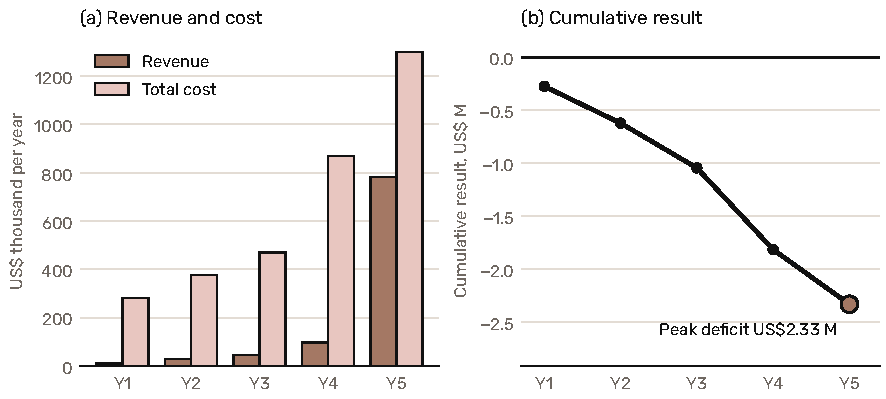
\includegraphics[width=\textwidth]{figures/f5-projection.pdf}
\caption{Five-year projection and cumulative result (model output; no operating profit in the horizon)}\label{fig:f5}
\end{figure}

\begin{table}[tbp]
\caption{Company-level sensitivity (model output; the rows are defined in the text)}\label{tab:company-sens}
% Company-level sensitivity (python/company_sensitivity.py). All amounts US$ thousand. Caption and label tab:company-sens: qa-se.
\ctnumcols{5}
\begin{tabularx}{\textwidth}{WVVVVV}
\toprule
\ctheaderrow\cthead{Scenario (US\$ thousand)} & \cthead{Y5 revenue} & \cthead{Y5 result} & \cthead{Peak deficit} & \cthead{Ask} & \cthead{Break-even clients}\\
\midrule
Base case & 458 & $-$998 & 3\,249 & 3\,899 & 44\\
Pilot-to-paying 35\% & 345 & $-$1\,088 & 3\,362 & 4\,035 & 44\\
Orders 500\,k & 296 & $-$1\,127 & 3\,377 & 4\,053 & 88\\
Low-touch 250\,k & 276 & $-$1\,143 & 3\,393 & 4\,072 & 101\\
Europe +1 yr & 104 & $-$1\,208 & 3\,348 & 4\,017 & 42\\
Scan cost $\times$2 & 458 & $-$1\,087 & 3\,373 & 4\,047 & 61\\
Europe in yr 3 & 998 & $-$571 & 3\,352 & 4\,023 & 44\\
\bottomrule
\end{tabularx}

\end{table}

The rows of Table~\ref{tab:company-sens} are defined as follows. Pilot-to-paying 35\% scales paying clients by 0.35/0.50. Orders 500\,k replaces the one million orders per European client. Europe one year later sets entry to year 5, with 36 European pilots and no paying European clients in year 5. Scan cost doubled doubles the cost per scan and the scan part (\usd{600}) of the direct pilot cost. The peak deficit is the end-of-year-5 value, and the ask is the deficit plus 20\%. Run-rate break-even stays outside the model horizon in all five rows. The table shows that every change moves the ask up and none brings break-even inside the horizon. Conversion at 35\% lifts the ask from \usd{2,798,850} to \usd{3,027,135} and cuts year-5 revenue from \usd{782,000} to \usd{571,400}. Half the orders per European client gives \usd{458,000} of revenue and an ask of \usd{3,106,650}. A one-year delay of Europe is the worst case: year-5 revenue falls to \usd{104,000} and the ask rises to \usd{3,423,450}. Doubling the scan cost raises the ask to \usd{3,028,620} and leaves revenue unchanged.

\section{Assumptions}\label{sec:assumptions}
Table~\ref{tab:assumptions} lists the inputs of this chapter with their class.

\begin{table}[tbp]
\caption{Main inputs of the financial plan}\label{tab:assumptions}
\begin{tabularx}{\textwidth}{XRlX}
\toprule
\ctheaderrow\cthead{Input} & \cthead{Value} & \cthead{Class} & \cthead{Basis}\\
\midrule
Return rate $r$ & \pct{24.4} & Sourced & US survey~\cite{coresight2023}\\
Return cost, share of prime cost & \pct{17} & Sourced & One retailer~\cite{gustafsson2021}\\
Order value & \usd{80} & Assumed & Mid-market basket\\
Fit-related share $\varphi$ & \pct{40} & Assumed & Below the 53\% who name fit\\
Reduction $\rho$ & \pct{15} & Assumed & Below Gustafsson scenarios\\
Price, Growth / Enterprise & \usd{0.04} / \usd{0.03} & Assumed & 40\% / 30\% of value\\
Cost to serve per order & \usd{0.0075} & Assumed & Scan \usd{0.03} on 25\% of orders\\
Cost per person-year & \usd{90,000} & Assumed & Blended\\
Orders per client, Israel / Europe & 250,000 / 1,000,000 & Derived / Assumed & Client bands\\
Funding buffer & \pct{20} & Assumed & Judgement\\
\bottomrule
\end{tabularx}
\end{table}

Most of the inputs in Table~\ref{tab:assumptions} are assumed, and only the return rate and the return-cost ratio are sourced, both from a single study each. The inputs that move the funding ask most in Table~\ref{tab:company-sens} are the year of Europe entry and the orders per European client; conversion at 35\% and a doubled scan cost each add about \usd{0.23} million. The pilot of Chapter~\ref{ch:gtm} can test the effect $\rho$, but it cannot test the other inputs, which stay open until the first clients have paid for a full year.

\section{Sensitivity to the pilot result}\label{sec:sensitivity}
Figure~\ref{fig:f6} shows the retailer's economics against the achieved effect $\rho$. The retailer breaks even at $\rho=\derived{6.03\%}$ on the Growth price and \derived{4.52\%} on the Enterprise price. At zero effect the client pays for nothing, so the pilot gate must stop the rollout. This answers the risk raised by a large study that found size-finder users slightly more likely to return~\cite{patel2025}. The same study reports a customer lifetime value 7.51\% higher in the next quarter for each unit increase in size-finder use. We mention it as a possible second lever and leave it out of the base case.

\begin{figure}[tbp]
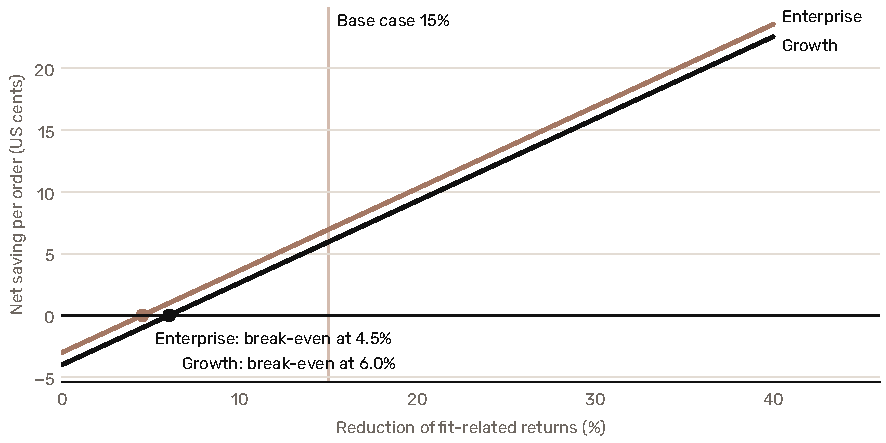
\includegraphics[width=\textwidth]{figures/f6-retailer-economics.pdf}
\caption{Retailer's economics against the achieved reduction $\rho$ (derived)}\label{fig:f6}
\end{figure}

\ctchapterend

\chapter{Risks}\label{ch:risks}

\section{The register}\label{sec:register}
Six risks are rated for likelihood and impact on a scale of 1 to 5, and each has a mitigation (Figure~\ref{fig:f7}, Table~\ref{tab:risks}). All scores are \assumed{assumed} judgements.

\begin{figure}[tbp]
\centering
% F7: risk heat matrix, likelihood x impact (1-5). Scores are assumed (assumptions.csv A29).
% No caption/label here: the chapter owns them (fig:f7). Numbers follow the row order of tab:risks:
% 1 privacy (L3,I4)  2 null effect (3,5)  3 edge sizes (3,3)  4 platform (3,4)  5 scan cost (2,4)  6 Europe (3,5)
\begin{tikzpicture}[x=1cm,y=0.8cm]
  \foreach \l in {1,...,5}{ \foreach \i in {1,...,5}{
    \pgfmathtruncatemacro{\s}{\l*\i}
    \pgfmathtruncatemacro{\c}{\s<=4 ? 1 : (\s<=8 ? 2 : (\s<=12 ? 3 : (\s<=16 ? 4 : 5)))}
    \node[ct cell \c,minimum width=1.4cm,minimum height=0.8cm,anchor=south west,inner sep=0pt] at (\i*1.4-1.4,\l*0.8-0.8) {};
  }}
  \foreach \i in {1,...,5}{ \node[ct label] at (\i*1.4-0.7,-0.35) {\i}; \node[ct label,anchor=east] at (-0.05,\i*0.8-0.4) {\i}; }
  \node[ct label] at (3.5,-1) {Impact};
  \node[ct label,rotate=90] at (-0.8,2) {Likelihood};
  \tikzset{rk/.style={circle,fill=white,draw=ink,minimum size=5mm,inner sep=0pt,font=\ctsmallfont\bfseries}}
  % cell centres: impact i at x=1.4 i-0.7, likelihood l at y=0.8 l-0.4
  \node[rk] at (3.5,2.0) {3};
  \node[rk] at (4.62,2.0) {1}; \node[rk] at (5.18,2.0) {4};
  \node[rk] at (6.02,2.0) {2}; \node[rk] at (6.58,2.0) {6};
  \node[rk] at (4.9,1.2) {5};
  \node[ct label,anchor=west,align=left] at (8,2)
    {1~Israeli privacy law\\2~Null pilot effect\\3~Edge sizes\\4~Platform (Google)\\5~Scan unit cost\\6~Europe entry slower};
\end{tikzpicture}

\caption{Risk matrix: likelihood against impact (scores assumed)}\label{fig:f7}
\end{figure}

\section{Israeli privacy law, with GDPR secondary}\label{sec:legal-risk}
The primary legal risk is Israel's Privacy Protection Law as amended by Amendment 13, in force since 14 August 2025~\cite{il_amend13_2024}. A biometric identifier is data of special sensitivity when it is used or intended to identify a person~\cite{il_ppl_en}, and a database holding such data about more than 100,000 people triggers a duty to notify the Authority. The mitigation is design: ClosetTwin scans for fit and never for identification, collects the minimum, and runs a consent flow and a compliance milestone before any pilot data are collected. Three limits apply. Explicit consent is our design choice, since the law defines consent as explicit or implied. Whether body measurements count as health data is an open legal question, so we treat it as a design risk and draw no conclusion. And the Authority's data-minimization opinion is a 2021 draft~\cite{ppa_data_minimization2021}. Article 9 of the GDPR~\cite{gdpr2016} is secondary: it applies when Israeli sites sell to EU customers and in the Europe stage.

\section{Null pilot effect and weak conversion}\label{sec:null-effect}
A size tool can fail to cut returns. The largest study in our sources found users slightly more likely to return an item~\cite{patel2025}. The pilot gate of Chapter~\ref{ch:gtm} is the mitigation: no rollout without a pass. The assumed 50\% conversion of pilots to paying clients is the weakest link of the plan, and it is named here with this risk.

\section{Accuracy at edge sizes}\label{sec:edge-sizes}
A supervised size model reached 89.66\% accuracy on scan data but failed at edge sizes~\cite{alhassawi2025}. Rare-size shoppers therefore get a fallback to the retailer's size chart.

\section{Platform risk, scan cost and slower Europe entry}\label{sec:platform-risk}
Google offers free try-on~\cite{google2023tryon}, so a retailer may rely on the platform. Our answer, the combination of garment data and preference, is still a hypothesis. If a scan costs more than about \usd{0.1} to serve, the model fails, and one vendor's list price of about \usd{2.00} per scan~\cite{threedlook_pricing} is 67 times our assumed \usd{0.03}, so we need an in-house scan. Last, nearly all revenue depends on Europe entry, because Israel's fee pool is about \usd{198,000} a year. If entry is slower than planned, the funding ask rises.

\begin{table}[tbp]
\caption{Mitigations (likelihood, impact; assumed)}\label{tab:risks}
\begin{tabularx}{\textwidth}{lRX}
\toprule
\ctheaderrow\cthead{Risk} & \cthead{L, I} & \cthead{Mitigation and trigger}\\
\midrule
Israeli privacy law (GDPR secondary) & 3, 4 & Scan for fit only; compliance milestone before pilot data\\
Null pilot effect, weak conversion & 3, 5 & Pilot gate; stop if the pass line is missed\\
Accuracy at edge sizes & 3, 3 & Fallback to size chart\\
Platform risk (Google) & 3, 4 & Garment data and preference integration\\
Scan unit cost above model & 2, 4 & In-house scan; stop above \usd{0.1} per scan\\
Europe entry slower than plan & 3, 5 & Stage gate at the Israeli pilot result\\
\bottomrule
\end{tabularx}
\end{table}
\ctchapterend

\chapter{Conclusion}\label{ch:conclusion}

\section{The case}\label{sec:case}
Returns cost retailers hundreds of billions of dollars a year, with estimates from \usd{685} to \usd{890} billion for 2024~\cite{appriss2024,nrf2024}, and size and fit uncertainty is a leading cause~\cite{coresight2023}. ClosetTwin's answer, a fit tool built on a body scan, garment data and stated preference, is a hypothesis and not a result. Its strength is that a four-week, shopper-level pilot can accept or reject it cheaply, and a retailer breaks even at an effect of 4.5\% to 6.0\%, below the 10\% pass line we set.

\section{The ask}\label{sec:ask}
We ask for a seed of about \derived{\usd{2.8}} million: the cumulative deficit of \usd{2.33} million at the end of year 5 plus a 20\% buffer. It funds the Israeli pilots, the Europe entry in year 4 and the run to run-rate break-even in year 6. This is a reference-market-then-expansion plan. Israel's addressable fee pool is only about \usd{198,000} a year, so Israel proves the product and Europe carries the revenue. The plan shows no operating profit within five years, and we say so plainly.

\section{Next steps}\label{sec:next}
The Israeli pilots come first, after the privacy compliance milestone and before any pilot data are collected. Nothing else is funded until a large-retailer pilot passes the 10\% line. If none passes, we stop and do not scale.
\ctchapterend


\ctreferences

\ctunnumbered{Appendix A: Code of the retailer-economics chart}
\label{app:code}
This appendix reproduces the Python script that draws Figure~\ref{fig:f6}, so the chart can be regenerated from the model outputs.
\pythonbox{python/appendix_f6_code.py}

\end{document}
